\section{コサイン類似度を用いたi-vectorの性質の調査}
\label{section:pre_cos}
発話データの長さを変更してi-vectorを抽出、コサイン類似度を算出してヒストグラムにすることで、発話の長さによるi-vectorの性質を調査する。
\subsection{使用する音声データ}
\label{section:detail_ATR}
本調査では、UBMモデルの学習データおよびコサイン類似度を用いたi-vectorの性質の調査に読み上げ音声\cite{ATR}を使用した。読み上げ音声には、男女各110人×50発話分が収録されている。

\subsection{コサイン類似度の算出条件}
対象の音声データからある発話を取り出し、それ以外の発話とのi-vectorのコサイン類似度を算出する。それを同一話者の発話間の場合と異なる話者の発話間の2つの場合に分けてヒストグラムに表し、コサイン類似度の性質の調査を行った。\par
i-vectorの抽出には、ALIZEとLIR RALを用いる。読み上げ音声に収録されている各発話データからi-vectorを抽出する。発話データから抽出する音響特徴パラメータを表\ref{iv_feature}に示す。また混合数は32とした。

\begin{table}[H]
  \begin{center}
    \caption{使用する音響特徴パラメータ}
    \label{iv_feature}
    \begin{tabular}{|c||c|} \hline
      特徴量 & 次元数\\ \hline
      MFCC & 19  \\ 
      POW & 1  \\ 
      $\Delta$MFCC & 19 \\ 
      $\Delta$POW & 1 \\ 
      $\Delta\Delta$MFCC & 19 \\ 
      $\Delta\Delta$POW & 1 \\ \hline
      計 & 60 \\ \hline
    \end{tabular}
  \end{center}
\end{table}

本研究では、音響特徴量のひとつとしてメル周波数ケプストラム係数(MFCC)を用いる。メル周波数ケプストラム係数(Mel - Frequency Cepstrum Coefficient : MFCC)とは、メル周波数という人間の音の高低に対する感覚尺度を考慮した特徴量であり、音声スペクトルから係数スペクトルを抽出したものである。これは一般的に、音声の特徴を抽出するパラメータとして用いられる。[5]

\subsection{長い音声データから抽出したi-vectorの性質}
本節では、比較的長い音声データとして、20秒間の音声データからi-vectorを抽出した。その結果、図\ref{fig:iv_same_long}より、同一話者の発話間の場合はコサイン類似度が高い値に多く分布し、図\ref{fig:iv_other_long}より、異なる話者の発話間の場合はコサイン類似度が全体的に分布していることが分かる。\par
これより、比較的長い音声データでは、コサイン類似度の値が高いほど、i-vectorを照合した発話の話者が同一の話者である確率が高いということが分かる。

\begin{figure}[H]
  \begin{center}
    \includegraphics{../../image/same_sp_long.eps}
  \end{center}
  \caption{長い音声データから抽出した同一話者間のi-vectorのコサイン類似度 \label{fig:iv_same_long}}
\end{figure}

\begin{figure}[H]
  \begin{center}
    \includegraphics{../../image/other_sp_long.eps}
  \end{center}
  \caption{長い音声データから抽出した異なる話者間のi-vectorのコサイン類似度 \label{fig:iv_other_long}}
\end{figure}

\subsection{非常に短い音声データから抽出したi-vectorの性質}
本節では、非常に音声データとして、0.3秒間の音声データからi-vectorを抽出した。その結果を図\ref{fig:iv_same_short}と図\ref{fig:iv_other_short}に示す。\par

\begin{figure}[H]
  \begin{center}
    \includegraphics{../../image/same_sp_short_0_3.eps}
  \end{center}
  \caption{非常に短い音声データから抽出した同一話者間のi-vectorのコサイン類似度 \label{fig:iv_same_short}}
\end{figure}

\begin{figure}[H]
  \begin{center}
    \includegraphics{../../image/other_sp_short_0_3.eps}
  \end{center}
  \caption{非常に短い音声データから抽出した異なる話者間のi-vectorのコサイン類似度 \label{fig:iv_other_short}} 
\end{figure}

非常に短い音声データから抽出したi-vectorは同一話者間ではコサイン類似度が0.2付近、異なる話者間では0付近に多くのデータが集まっている。しかし、同一話者間のコサイン類似度と異なる話者間のコサイン類似度のヒストグラムは非常に似た形をしており、本検証で抽出されたi-vectorでは話者の識別をすることは非常に難しい。これより、i-vectorを用いた話者照合、話者識別を行う場合はできるだけ長い発話データを用意することが必要である。
